% Options for packages loaded elsewhere
\PassOptionsToPackage{unicode}{hyperref}
\PassOptionsToPackage{hyphens}{url}
%
\documentclass[
]{book}
\title{R과 통계분석}
\author{박동련}
\date{2022-02-12}

\usepackage{amsmath,amssymb}
\usepackage{lmodern}
\usepackage{iftex}
\ifPDFTeX
  \usepackage[T1]{fontenc}
  \usepackage[utf8]{inputenc}
  \usepackage{textcomp} % provide euro and other symbols
\else % if luatex or xetex
  \usepackage{unicode-math}
  \defaultfontfeatures{Scale=MatchLowercase}
  \defaultfontfeatures[\rmfamily]{Ligatures=TeX,Scale=1}
\fi
% Use upquote if available, for straight quotes in verbatim environments
\IfFileExists{upquote.sty}{\usepackage{upquote}}{}
\IfFileExists{microtype.sty}{% use microtype if available
  \usepackage[]{microtype}
  \UseMicrotypeSet[protrusion]{basicmath} % disable protrusion for tt fonts
}{}
\makeatletter
\@ifundefined{KOMAClassName}{% if non-KOMA class
  \IfFileExists{parskip.sty}{%
    \usepackage{parskip}
  }{% else
    \setlength{\parindent}{0pt}
    \setlength{\parskip}{6pt plus 2pt minus 1pt}}
}{% if KOMA class
  \KOMAoptions{parskip=half}}
\makeatother
\usepackage{xcolor}
\IfFileExists{xurl.sty}{\usepackage{xurl}}{} % add URL line breaks if available
\IfFileExists{bookmark.sty}{\usepackage{bookmark}}{\usepackage{hyperref}}
\hypersetup{
  pdftitle={R과 통계분석},
  pdfauthor={박동련},
  hidelinks,
  pdfcreator={LaTeX via pandoc}}
\urlstyle{same} % disable monospaced font for URLs
\usepackage{color}
\usepackage{fancyvrb}
\newcommand{\VerbBar}{|}
\newcommand{\VERB}{\Verb[commandchars=\\\{\}]}
\DefineVerbatimEnvironment{Highlighting}{Verbatim}{commandchars=\\\{\}}
% Add ',fontsize=\small' for more characters per line
\usepackage{framed}
\definecolor{shadecolor}{RGB}{248,248,248}
\newenvironment{Shaded}{\begin{snugshade}}{\end{snugshade}}
\newcommand{\AlertTok}[1]{\textcolor[rgb]{0.94,0.16,0.16}{#1}}
\newcommand{\AnnotationTok}[1]{\textcolor[rgb]{0.56,0.35,0.01}{\textbf{\textit{#1}}}}
\newcommand{\AttributeTok}[1]{\textcolor[rgb]{0.77,0.63,0.00}{#1}}
\newcommand{\BaseNTok}[1]{\textcolor[rgb]{0.00,0.00,0.81}{#1}}
\newcommand{\BuiltInTok}[1]{#1}
\newcommand{\CharTok}[1]{\textcolor[rgb]{0.31,0.60,0.02}{#1}}
\newcommand{\CommentTok}[1]{\textcolor[rgb]{0.56,0.35,0.01}{\textit{#1}}}
\newcommand{\CommentVarTok}[1]{\textcolor[rgb]{0.56,0.35,0.01}{\textbf{\textit{#1}}}}
\newcommand{\ConstantTok}[1]{\textcolor[rgb]{0.00,0.00,0.00}{#1}}
\newcommand{\ControlFlowTok}[1]{\textcolor[rgb]{0.13,0.29,0.53}{\textbf{#1}}}
\newcommand{\DataTypeTok}[1]{\textcolor[rgb]{0.13,0.29,0.53}{#1}}
\newcommand{\DecValTok}[1]{\textcolor[rgb]{0.00,0.00,0.81}{#1}}
\newcommand{\DocumentationTok}[1]{\textcolor[rgb]{0.56,0.35,0.01}{\textbf{\textit{#1}}}}
\newcommand{\ErrorTok}[1]{\textcolor[rgb]{0.64,0.00,0.00}{\textbf{#1}}}
\newcommand{\ExtensionTok}[1]{#1}
\newcommand{\FloatTok}[1]{\textcolor[rgb]{0.00,0.00,0.81}{#1}}
\newcommand{\FunctionTok}[1]{\textcolor[rgb]{0.00,0.00,0.00}{#1}}
\newcommand{\ImportTok}[1]{#1}
\newcommand{\InformationTok}[1]{\textcolor[rgb]{0.56,0.35,0.01}{\textbf{\textit{#1}}}}
\newcommand{\KeywordTok}[1]{\textcolor[rgb]{0.13,0.29,0.53}{\textbf{#1}}}
\newcommand{\NormalTok}[1]{#1}
\newcommand{\OperatorTok}[1]{\textcolor[rgb]{0.81,0.36,0.00}{\textbf{#1}}}
\newcommand{\OtherTok}[1]{\textcolor[rgb]{0.56,0.35,0.01}{#1}}
\newcommand{\PreprocessorTok}[1]{\textcolor[rgb]{0.56,0.35,0.01}{\textit{#1}}}
\newcommand{\RegionMarkerTok}[1]{#1}
\newcommand{\SpecialCharTok}[1]{\textcolor[rgb]{0.00,0.00,0.00}{#1}}
\newcommand{\SpecialStringTok}[1]{\textcolor[rgb]{0.31,0.60,0.02}{#1}}
\newcommand{\StringTok}[1]{\textcolor[rgb]{0.31,0.60,0.02}{#1}}
\newcommand{\VariableTok}[1]{\textcolor[rgb]{0.00,0.00,0.00}{#1}}
\newcommand{\VerbatimStringTok}[1]{\textcolor[rgb]{0.31,0.60,0.02}{#1}}
\newcommand{\WarningTok}[1]{\textcolor[rgb]{0.56,0.35,0.01}{\textbf{\textit{#1}}}}
\usepackage{longtable,booktabs,array}
\usepackage{calc} % for calculating minipage widths
% Correct order of tables after \paragraph or \subparagraph
\usepackage{etoolbox}
\makeatletter
\patchcmd\longtable{\par}{\if@noskipsec\mbox{}\fi\par}{}{}
\makeatother
% Allow footnotes in longtable head/foot
\IfFileExists{footnotehyper.sty}{\usepackage{footnotehyper}}{\usepackage{footnote}}
\makesavenoteenv{longtable}
\usepackage{graphicx}
\makeatletter
\def\maxwidth{\ifdim\Gin@nat@width>\linewidth\linewidth\else\Gin@nat@width\fi}
\def\maxheight{\ifdim\Gin@nat@height>\textheight\textheight\else\Gin@nat@height\fi}
\makeatother
% Scale images if necessary, so that they will not overflow the page
% margins by default, and it is still possible to overwrite the defaults
% using explicit options in \includegraphics[width, height, ...]{}
\setkeys{Gin}{width=\maxwidth,height=\maxheight,keepaspectratio}
% Set default figure placement to htbp
\makeatletter
\def\fps@figure{htbp}
\makeatother
\setlength{\emergencystretch}{3em} % prevent overfull lines
\providecommand{\tightlist}{%
  \setlength{\itemsep}{0pt}\setlength{\parskip}{0pt}}
\setcounter{secnumdepth}{5}
\usepackage{booktabs}
\ifLuaTeX
  \usepackage{selnolig}  % disable illegal ligatures
\fi
\usepackage[]{natbib}
\bibliographystyle{plainnat}

\begin{document}
\maketitle

{
\setcounter{tocdepth}{1}
\tableofcontents
}
\hypertarget{uxc18cuxac1cuxd558uxae30}{%
\chapter*{소개하기}\label{uxc18cuxac1cuxd558uxae30}}
\addcontentsline{toc}{chapter}{소개하기}


\includegraphics{Figure/cover.jpg}

\hypertarget{r-uxc2dcuxc791uxd558uxae30}{%
\chapter{R 시작하기}\label{r-uxc2dcuxc791uxd558uxae30}}

Placeholder

\hypertarget{ruxc758-uxc18cuxac1c}{%
\section{R의 소개}\label{ruxc758-uxc18cuxac1c}}

\hypertarget{ruxc758-uxc124uxce58}{%
\section{R의 설치}\label{ruxc758-uxc124uxce58}}

\hypertarget{rstudiouxc758-uxc124uxce58-uxbc0f-ruxc758-uxc2e4uxd589}{%
\section{RStudio의 설치 및 R의 실행}\label{rstudiouxc758-uxc124uxce58-uxbc0f-ruxc758-uxc2e4uxd589}}

\hypertarget{uxc791uxc5c5uxacf5uxac04}{%
\section{작업공간}\label{uxc791uxc5c5uxacf5uxac04}}

\hypertarget{uxc2a4uxd06cuxb9bduxd2b8-uxd30cuxc77cuxc758-uxd65cuxc6a9}{%
\section{스크립트 파일의 활용}\label{uxc2a4uxd06cuxb9bduxd2b8-uxd30cuxc77cuxc758-uxd65cuxc6a9}}

\hypertarget{section-batch}{%
\section{일괄처리}\label{section-batch}}

\hypertarget{section-package}{%
\section{R의 확장: 패키지}\label{section-package}}

\hypertarget{uxd328uxd0a4uxc9c0uxc758-uxc885uxb958}{%
\subsection{패키지의 종류}\label{uxd328uxd0a4uxc9c0uxc758-uxc885uxb958}}

\hypertarget{uxd328uxd0a4uxc9c0uxc758-uxc124uxce58-uxbc0f-uxc0acuxc6a9}{%
\subsection{패키지의 설치 및 사용}\label{uxd328uxd0a4uxc9c0uxc758-uxc124uxce58-uxbc0f-uxc0acuxc6a9}}

\hypertarget{uxd328uxd0a4uxc9c0-tidyverseuxc758-uxc18cuxac1c}{%
\subsection{패키지 tidyverse의 소개}\label{uxd328uxd0a4uxc9c0-tidyverseuxc758-uxc18cuxac1c}}

\hypertarget{data-structure}{%
\chapter{R 데이터 구조}\label{data-structure}}

Placeholder

\hypertarget{uxbca1uxd130}{%
\section{벡터}\label{uxbca1uxd130}}

\hypertarget{uxbca1uxd130uxc758-uxae30uxbcf8-uxd2b9uxc131}{%
\subsection{벡터의 기본 특성}\label{uxbca1uxd130uxc758-uxae30uxbcf8-uxd2b9uxc131}}

\hypertarget{uxb2e4uxc591uxd55c-uxd615uxd0dcuxb97c-uxac16uxb294-uxbca1uxd130uxc758-uxc0dduxc131}{%
\subsection{다양한 형태를 갖는 벡터의 생성}\label{uxb2e4uxc591uxd55c-uxd615uxd0dcuxb97c-uxac16uxb294-uxbca1uxd130uxc758-uxc0dduxc131}}

\hypertarget{uxbca1uxd130uxc5d0-uxb370uxc774uxd130-uxcd94uxac00-uxbc0f-uxbca1uxd130uxb4e4uxc758-uxacb0uxd569}{%
\subsubsection{벡터에 데이터 추가 및 벡터들의 결합}\label{uxbca1uxd130uxc5d0-uxb370uxc774uxd130-uxcd94uxac00-uxbc0f-uxbca1uxd130uxb4e4uxc758-uxacb0uxd569}}

\hypertarget{uxc77cuxc815uxd55c-uxad6cuxc870uxb97c-uxac16uxb294-uxbca1uxd130uxc758-uxc0dduxc131}{%
\subsubsection{일정한 구조를 갖는 벡터의 생성}\label{uxc77cuxc815uxd55c-uxad6cuxc870uxb97c-uxac16uxb294-uxbca1uxd130uxc758-uxc0dduxc131}}

\hypertarget{uxbb38uxc790uxc5f4uxc744-uxc704uxd55c-uxd568uxc218}{%
\subsection{문자열을 위한 함수}\label{uxbb38uxc790uxc5f4uxc744-uxc704uxd55c-uxd568uxc218}}

\hypertarget{uxbca1uxd130uxc758-uxc5f0uxc0b0}{%
\subsection{벡터의 연산}\label{uxbca1uxd130uxc758-uxc5f0uxc0b0}}

\hypertarget{uxbca1uxd130uxc758-uxbe44uxad50}{%
\subsection{벡터의 비교}\label{uxbca1uxd130uxc758-uxbe44uxad50}}

\hypertarget{uxbca1uxd130uxc758-uxc778uxb371uxc2f1}{%
\subsection{벡터의 인덱싱}\label{uxbca1uxd130uxc758-uxc778uxb371uxc2f1}}

\hypertarget{uxc694uxc778}{%
\section{요인}\label{uxc694uxc778}}

\hypertarget{uxc694uxc778uxc758-uxae30uxbcf8-uxd2b9uxc131}{%
\subsection{요인의 기본 특성}\label{uxc694uxc778uxc758-uxae30uxbcf8-uxd2b9uxc131}}

\hypertarget{uxc22buxc790uxd615-uxbca1uxd130uxb97c-uxc694uxc778uxc73cuxb85c-uxbcc0uxd658}{%
\subsection{숫자형 벡터를 요인으로 변환}\label{uxc22buxc790uxd615-uxbca1uxd130uxb97c-uxc694uxc778uxc73cuxb85c-uxbcc0uxd658}}

\hypertarget{uxb0a0uxc9dc}{%
\section{날짜}\label{uxb0a0uxc9dc}}

\hypertarget{uxd589uxb82c-uxbc0f-uxbc30uxc5f4}{%
\section{행렬 및 배열}\label{uxd589uxb82c-uxbc0f-uxbc30uxc5f4}}

\hypertarget{uxd589uxb82cuxacfc-uxbc30uxc5f4uxc758-uxae30uxbcf8-uxd2b9uxc131}{%
\subsection{행렬과 배열의 기본 특성}\label{uxd589uxb82cuxacfc-uxbc30uxc5f4uxc758-uxae30uxbcf8-uxd2b9uxc131}}

\hypertarget{uxd589uxb82cuxc758-uxc5f0uxc0b0}{%
\subsection{행렬의 연산}\label{uxd589uxb82cuxc758-uxc5f0uxc0b0}}

\hypertarget{section-dataframe}{%
\section{데이터 프레임}\label{section-dataframe}}

\hypertarget{uxb370uxc774uxd130-uxd504uxb808uxc784uxc758-uxc0dduxc131}{%
\subsection{데이터 프레임의 생성}\label{uxb370uxc774uxd130-uxd504uxb808uxc784uxc758-uxc0dduxc131}}

\hypertarget{uxb370uxc774uxd130-uxd504uxb808uxc784uxc758-uxc778uxb371uxc2f1}{%
\subsection{데이터 프레임의 인덱싱}\label{uxb370uxc774uxd130-uxd504uxb808uxc784uxc758-uxc778uxb371uxc2f1}}

\hypertarget{uxd568uxc218-with}{%
\subsection{\texorpdfstring{함수 \texttt{with()}}{함수 with()}}\label{uxd568uxc218-with}}

\hypertarget{tibble-uxac1cuxc120uxb41c-uxd615uxd0dcuxc758-uxb370uxc774uxd130-uxd504uxb808uxc784}{%
\section{Tibble: 개선된 형태의 데이터 프레임}\label{tibble-uxac1cuxc120uxb41c-uxd615uxd0dcuxc758-uxb370uxc774uxd130-uxd504uxb808uxc784}}

\hypertarget{tibble-uxc0dduxc131}{%
\subsection{Tibble 생성}\label{tibble-uxc0dduxc131}}

\hypertarget{tibbleuxacfc-uxc804uxd1b5uxc801uxc778-uxb370uxc774uxd130-uxd504uxb808uxc784uxc758-uxcc28uxc774}{%
\subsection{Tibble과 전통적인 데이터 프레임의 차이}\label{tibbleuxacfc-uxc804uxd1b5uxc801uxc778-uxb370uxc774uxd130-uxd504uxb808uxc784uxc758-uxcc28uxc774}}

\hypertarget{section-list}{%
\section{리스트}\label{section-list}}

\hypertarget{uxc5f0uxc2b5uxbb38uxc81c}{%
\section{연습문제}\label{uxc5f0uxc2b5uxbb38uxc81c}}

\begin{enumerate}
\def\labelenumi{\arabic{enumi}.}
\tightlist
\item
  데이터 프레임 \texttt{iris}는 세 가지 종류 붓꽃 \texttt{setosa} , \texttt{versicolor} , \texttt{virginica}의 꽃잎과 꽃받침의 길이와 폭을 측정한 자료이다. 각 종류별로 50송이를 측정하여 처음 50개 행에는 \texttt{setosa}, 51부터 100번째 행에는 \texttt{versicolor}, 마지막 50개 행에는 \texttt{viginica}의 측정값이 입력되어 있다.
\end{enumerate}

\begin{itemize}
\tightlist
\item
  \texttt{iris}의 1\textasciitilde3 행 51\textasciitilde53 행 101\textasciitilde103 행을 다음과 같이 출력해 보자.
\end{itemize}

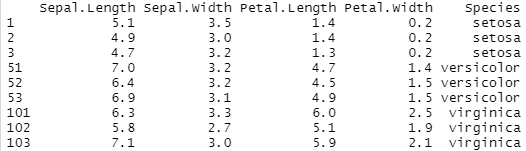
\includegraphics[width=5.20833in,height=\textheight]{Figure/ch2_ex_21_1.png}

\begin{itemize}
\item
  \texttt{iris}의 변수 \texttt{Sepal.Length}, \texttt{Sepal.Width}, \texttt{Petal.Length}, \texttt{Petal.Width}에는 꽃잎과 꽃받침의 길이와 폭을 측정한 결과가 입력되어 있다. 세 가지 붓꽃 종류별로 네 변수의 평균값을 각각 계산해 보자
\item
  150송이 중 \texttt{Petal.Width}의 값이 1 이하이고 \texttt{Petal.Length}가 4 이하인 붓꽃이 모두 몇 송이가 있는지 알아보자. 또한 세 종류의 붓꽃별로는 각각 몇 송이가 있는지 알아보자.
\end{itemize}

\begin{enumerate}
\def\labelenumi{\arabic{enumi}.}
\setcounter{enumi}{1}
\tightlist
\item
  데이터 프레임 \texttt{mtcars}는 1974년에 발행된 어떤 잡지에 소개된 32대 자동차의 연비와 관련된 자료이다.
\end{enumerate}

\begin{itemize}
\tightlist
\item
  숫자형 변수 \texttt{mpg}에 대한 다음의 조건으로 요인 \texttt{grade}를 생성해 보자. 단, \(\bar{x}\) 와 \(sd\) 는 변수 \texttt{mpg}의 평균 및 표준편차이다.
\end{itemize}

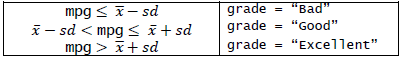
\includegraphics[width=3.125in,height=\textheight]{Figure/ch2_ex_21_2.PNG}

\begin{itemize}
\item
  \texttt{mtcars}의 행 이름을 데이터 프레임에 변수 이름 \texttt{model}로 추가해 보자
\item
  요인 \texttt{grade}가 \texttt{Excellent}인 자동차의 변수 \texttt{model}과 \texttt{mpg}의 값을 출력해 보자.
\item
  요인 \texttt{grade}가 \texttt{Bad}인 자동차들의 평균 \texttt{mpg} 값을 계산해 보자.
\end{itemize}

\hypertarget{uxb370uxc774uxd130-uxc785uxb825}{%
\chapter{데이터 입력}\label{uxb370uxc774uxd130-uxc785uxb825}}

Placeholder

\hypertarget{uxd14duxc2a4uxd2b8-uxd30cuxc77c-uxbd88uxb7ecuxc624uxae30-uxd328uxd0a4uxc9c0-readr-uxd568uxc218uxc758-uxd65cuxc6a9}{%
\section{\texorpdfstring{텍스트 파일 불러오기: 패키지 \texttt{readr} 함수의 활용}{텍스트 파일 불러오기: 패키지 readr 함수의 활용}}\label{uxd14duxc2a4uxd2b8-uxd30cuxc77c-uxbd88uxb7ecuxc624uxae30-uxd328uxd0a4uxc9c0-readr-uxd568uxc218uxc758-uxd65cuxc6a9}}

\hypertarget{uxd568uxc218-read_tableuxb85c-uxb370uxc774uxd130-uxd30cuxc77c-uxbd88uxb7ecuxc624uxae30}{%
\subsection{\texorpdfstring{함수 \texttt{read\_table()}로 데이터 파일 불러오기}{함수 read\_table()로 데이터 파일 불러오기}}\label{uxd568uxc218-read_tableuxb85c-uxb370uxc774uxd130-uxd30cuxc77c-uxbd88uxb7ecuxc624uxae30}}

\hypertarget{uxd568uxc218-read_csvuxb85c-csv-uxb370uxc774uxd130-uxd30cuxc77c-uxbd88uxb7ecuxc624uxae30}{%
\subsection{\texorpdfstring{함수 \texttt{read\_csv()}로 CSV 데이터 파일 불러오기}{함수 read\_csv()로 CSV 데이터 파일 불러오기}}\label{uxd568uxc218-read_csvuxb85c-csv-uxb370uxc774uxd130-uxd30cuxc77c-uxbd88uxb7ecuxc624uxae30}}

\hypertarget{uxd568uxc218-read_fwfuxb85c-uxace0uxc815-uxd3ecuxb9f7-uxad6cuxc870uxb97c-uxac16uxb294-uxb370uxc774uxd130-uxd30cuxc77c-uxbd88uxb7ecuxc624uxae30}{%
\subsection{\texorpdfstring{함수 \texttt{read\_fwf()}로 고정 포맷 구조를 갖는 데이터 파일 불러오기}{함수 read\_fwf()로 고정 포맷 구조를 갖는 데이터 파일 불러오기}}\label{uxd568uxc218-read_fwfuxb85c-uxace0uxc815-uxd3ecuxb9f7-uxad6cuxc870uxb97c-uxac16uxb294-uxb370uxc774uxd130-uxd30cuxc77c-uxbd88uxb7ecuxc624uxae30}}

\hypertarget{excel-uxd30cuxc77c-uxbd88uxb7ecuxc624uxae30}{%
\section{Excel 파일 불러오기}\label{excel-uxd30cuxc77c-uxbd88uxb7ecuxc624uxae30}}

\hypertarget{sas-uxb370uxc774uxd130-uxd30cuxc77c-uxbd88uxb7ecuxc624uxae30}{%
\section{SAS 데이터 파일 불러오기}\label{sas-uxb370uxc774uxd130-uxd30cuxc77c-uxbd88uxb7ecuxc624uxae30}}

\hypertarget{html-uxd14cuxc774uxbe14-uxbd88uxb7ecuxc624uxae30}{%
\section{HTML 테이블 불러오기}\label{html-uxd14cuxc774uxbe14-uxbd88uxb7ecuxc624uxae30}}

\hypertarget{dplyruxc5d0-uxc758uxd55c-uxb370uxc774uxd130-uxb2e4uxb4ecuxae30}{%
\chapter{\texorpdfstring{\texttt{dplyr}에 의한 데이터 다듬기}{dplyr에 의한 데이터 다듬기}}\label{dplyruxc5d0-uxc758uxd55c-uxb370uxc774uxd130-uxb2e4uxb4ecuxae30}}

Placeholder

\hypertarget{uxd589uxc744-uxc791uxc5c5-uxb300uxc0c1uxc73cuxb85c-uxd558uxb294-uxd568uxc218}{%
\section{행을 작업 대상으로 하는 함수}\label{uxd589uxc744-uxc791uxc5c5-uxb300uxc0c1uxc73cuxb85c-uxd558uxb294-uxd568uxc218}}

\hypertarget{uxc870uxac74uxc5d0-uxc758uxd55c-uxd589-uxc120uxd0dd-filter}{%
\subsection{\texorpdfstring{조건에 의한 행 선택: \texttt{filter()}}{조건에 의한 행 선택: filter()}}\label{uxc870uxac74uxc5d0-uxc758uxd55c-uxd589-uxc120uxd0dd-filter}}

\hypertarget{uxc704uxce58uxc5d0-uxc758uxd55c-uxd589-uxc120uxd0dd-slice-uxbc0f-uxadf8uxc640-uxad00uxb828uxb41c-uxd568uxc218}{%
\subsection{\texorpdfstring{위치에 의한 행 선택: \texttt{slice()} 및 그와 관련된 함수}{위치에 의한 행 선택: slice() 및 그와 관련된 함수}}\label{uxc704uxce58uxc5d0-uxc758uxd55c-uxd589-uxc120uxd0dd-slice-uxbc0f-uxadf8uxc640-uxad00uxb828uxb41c-uxd568uxc218}}

\hypertarget{uxd589uxc758-uxc815uxb82c-arrange}{%
\subsection{\texorpdfstring{행의 정렬: \texttt{arrange()}}{행의 정렬: arrange()}}\label{uxd589uxc758-uxc815uxb82c-arrange}}

\hypertarget{uxc911uxbcf5uxb41c-uxd589uxc758-uxc81cuxac70-distinct}{%
\subsection{\texorpdfstring{중복된 행의 제거: \texttt{distinct()}}{중복된 행의 제거: distinct()}}\label{uxc911uxbcf5uxb41c-uxd589uxc758-uxc81cuxac70-distinct}}

\hypertarget{uxc5f4uxc744-uxc791uxc5c5-uxb300uxc0c1uxc73cuxb85c-uxd558uxb294-uxd568uxc218}{%
\section{열을 작업 대상으로 하는 함수}\label{uxc5f4uxc744-uxc791uxc5c5-uxb300uxc0c1uxc73cuxb85c-uxd558uxb294-uxd568uxc218}}

\hypertarget{uxc5f4uxc758-uxc120uxd0dd-select}{%
\subsection{\texorpdfstring{열의 선택: \texttt{select()}}{열의 선택: select()}}\label{uxc5f4uxc758-uxc120uxd0dd-select}}

\hypertarget{uxc5f4-uxc774uxb984-uxbcc0uxacbd-renameuxacfc-rename_with}{%
\subsection{\texorpdfstring{열 이름 변경: \texttt{rename()}과 \texttt{rename\_with()}}{열 이름 변경: rename()과 rename\_with()}}\label{uxc5f4-uxc774uxb984-uxbcc0uxacbd-renameuxacfc-rename_with}}

\hypertarget{uxc5f4uxc758-uxc704uxce58-uxbcc0uxacbd-relocate}{%
\subsection{\texorpdfstring{열의 위치 변경: \texttt{relocate()}}{열의 위치 변경: relocate()}}\label{uxc5f4uxc758-uxc704uxce58-uxbcc0uxacbd-relocate}}

\hypertarget{uxc0c8uxb85cuxc6b4-uxc5f4uxc758-uxcd94uxac00-mutateuxc640-transmute}{%
\subsection{\texorpdfstring{새로운 열의 추가: \texttt{mutate()}와 \texttt{transmute()}}{새로운 열의 추가: mutate()와 transmute()}}\label{uxc0c8uxb85cuxc6b4-uxc5f4uxc758-uxcd94uxac00-mutateuxc640-transmute}}

\hypertarget{uxc5ecuxb7ec-uxd589-uxc790uxb8ccuxc758-uxc694uxc57d-summarise}{%
\section{\texorpdfstring{여러 행 자료의 요약: \texttt{summarise()}}{여러 행 자료의 요약: summarise()}}\label{uxc5ecuxb7ec-uxd589-uxc790uxb8ccuxc758-uxc694uxc57d-summarise}}

\hypertarget{uxadf8uxb8f9-uxb370uxc774uxd130-uxd504uxb808uxc784}{%
\section{그룹 데이터 프레임}\label{uxadf8uxb8f9-uxb370uxc774uxd130-uxd504uxb808uxc784}}

\hypertarget{uxadf8uxb8f9-uxb370uxc774uxd130-uxd504uxb808uxc784uxc758-uxc0dduxc131-group_by}{%
\subsection{\texorpdfstring{그룹 데이터 프레임의 생성: \texttt{group\_by()}}{그룹 데이터 프레임의 생성: group\_by()}}\label{uxadf8uxb8f9-uxb370uxc774uxd130-uxd504uxb808uxc784uxc758-uxc0dduxc131-group_by}}

\hypertarget{uxadf8uxb8f9-uxb370uxc774uxd130-uxd504uxb808uxc784uxc5d0uxc11c-uxae30uxbcf8-uxd568uxc218uxb4e4uxc758-uxc791uxb3d9-uxbc29uxc2dd}{%
\subsection{그룹 데이터 프레임에서 기본 함수들의 작동 방식}\label{uxadf8uxb8f9-uxb370uxc774uxd130-uxd504uxb808uxc784uxc5d0uxc11c-uxae30uxbcf8-uxd568uxc218uxb4e4uxc758-uxc791uxb3d9-uxbc29uxc2dd}}

\hypertarget{uxb2e4uxc218uxc758-uxc5f4uxc744-uxb300uxc0c1uxc73cuxb85c-uxd558uxb294-uxc791uxc5c5-across}{%
\section{\texorpdfstring{다수의 열을 대상으로 하는 작업: \texttt{across()}}{다수의 열을 대상으로 하는 작업: across()}}\label{uxb2e4uxc218uxc758-uxc5f4uxc744-uxb300uxc0c1uxc73cuxb85c-uxd558uxb294-uxc791uxc5c5-across}}

\hypertarget{uxd589-uxb2e8uxc704-uxc791uxc5c5-rowwise}{%
\section{\texorpdfstring{행 단위 작업: \texttt{rowwise()}}{행 단위 작업: rowwise()}}\label{uxd589-uxb2e8uxc704-uxc791uxc5c5-rowwise}}

\hypertarget{chapter-ggplot2}{%
\chapter{\texorpdfstring{\texttt{ggplot2}에 의한 자료 시각화}{ggplot2에 의한 자료 시각화}}\label{chapter-ggplot2}}

자료의 시각화(Visualization)란 자료의 구조를 꿰뚫어 볼 수 있는 명쾌한 그래프를 이용하는 자료 분석방법을 의미한다.
잘 그려진 그래프는 자료의 모습을 있는 그대로 보여 주는 유일한 분석방법이며,
다른 어떠한 분석기법에 의한 결과보다도 더 많은 정보를 전달해 줄 수 있는 방법이기도 하다.
Figure \ref{fig:barely}은 자료 시각화의 위력을 잘 보여주는 예로서 Cleveland(1993)에 의한 놀라운 발견이다.
1930년대 초 미네소타 주의 농경학자들이 보리 종류에 따른 수확량의 차이를 알아보기 위한 경작 실험을 실시하였다.
6군데 경작지에 10 종류 보리를 2년간 경작하였는데, Morris 지역만이 1932년의 수확량이 1931년의 수확량
보다 많다는 것을 알 수 있다. 6개 경작지가 모두 근처에 있다는 점을 고려해 보면 유독
Morris 지역에서만 다른 결과가 나왔다는 것이 상당히 의심스럽다고 할 수 있으며, 데이터
가 바뀌었을 가능성을 생각해 볼 수 있는 상황이다.

\begin{verbatim}
-- Attaching packages --------------------------------------- tidyverse 1.3.1 --
v ggplot2 3.3.5     v purrr   0.3.4
v tibble  3.1.6     v dplyr   1.0.7
v tidyr   1.1.4     v stringr 1.4.0
v readr   2.1.1     v forcats 0.5.1
-- Conflicts ------------------------------------------ tidyverse_conflicts() --
x dplyr::filter() masks stats::filter()
x dplyr::lag()    masks stats::lag()
\end{verbatim}

\begin{figure}
\centering
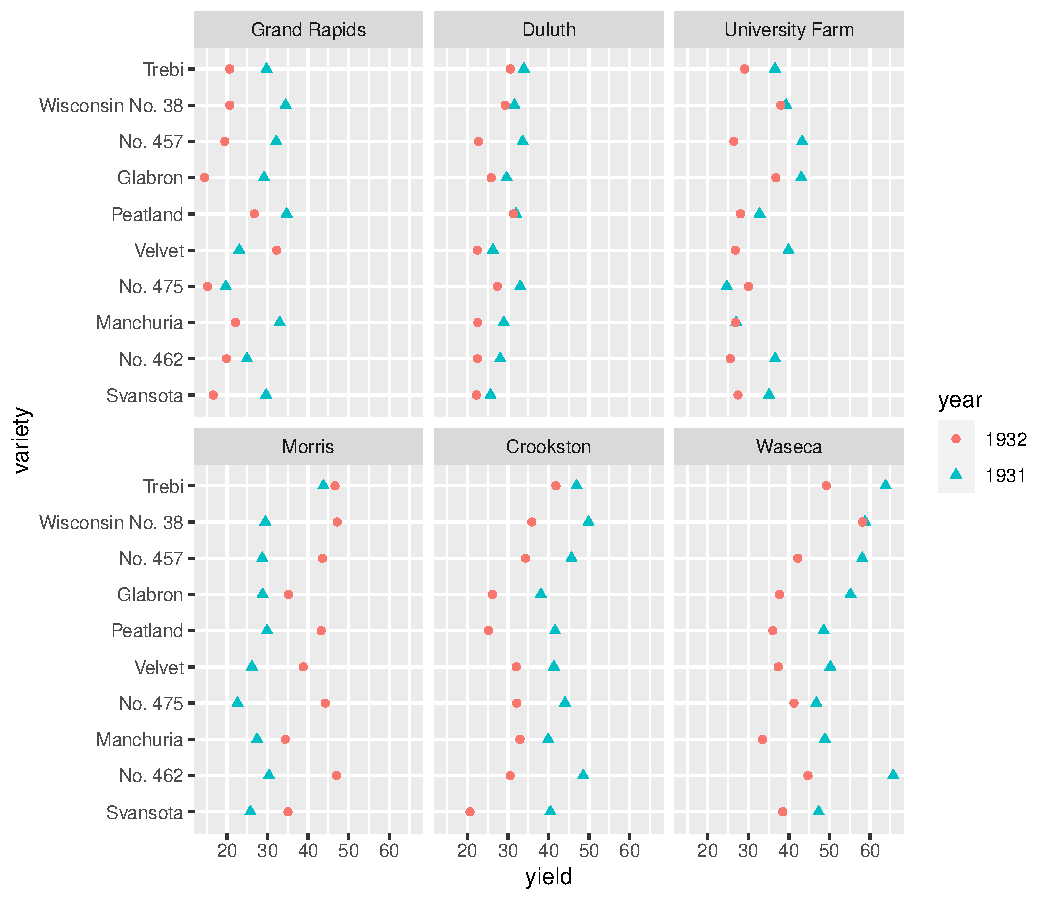
\includegraphics{_main_files/figure-latex/barely-1.pdf}
\caption{\label{fig:barely}보리 자료에 대한 다중 패널 점그림}
\end{figure}

자료 시각화에 특히 강점이 있는 R에는 몇 가지의 그래프 작성 시스템이 있다. 함수 \texttt{plot()} 등이 속해 있는
\texttt{base\ graphics}도 그 중 하나인데, 이들 그래프 작성 시스템 중 가장 효과적이고 여러 면에서 우수한 시스템이 바로 \texttt{ggplot2}라고 할 수 있다.
그래프 작성에 일관된 규칙이 있어서 복잡한 상황에서도 쉽게 확장이 가능하다는 것이 큰 장점 중 하나이다.

패키지 \texttt{ggplot2}도 core tidyverse에 속해있기 때문에 \texttt{library(tidyverse)}를 먼저 실행해 주면 사용할 수 있다.

\hypertarget{ggplot2-uxc2dcuxc791uxd558uxae30}{%
\section{\texorpdfstring{\texttt{ggplot2} 시작하기}{ggplot2 시작하기}}\label{ggplot2-uxc2dcuxc791uxd558uxae30}}

패키지 \texttt{ggplot2}에 있는 데이터 프레임 \texttt{mpg}의 변수 \texttt{displ}과 \texttt{hwy}의 관계를 산점도로 나타내보자.
변수 \texttt{displ}은 리터 단위의 배기량이고, \texttt{hwy}는 고속도로 연비이다.

\begin{Shaded}
\begin{Highlighting}[]
\SpecialCharTok{\textgreater{}} \FunctionTok{ggplot}\NormalTok{(}\AttributeTok{data =}\NormalTok{ mpg) }\SpecialCharTok{+}
\SpecialCharTok{+}   \FunctionTok{geom\_point}\NormalTok{(}\AttributeTok{mapping =} \FunctionTok{aes}\NormalTok{(}\AttributeTok{x =}\NormalTok{ displ, }\AttributeTok{y =}\NormalTok{ hwy))}
\end{Highlighting}
\end{Shaded}

\begin{figure}
\centering
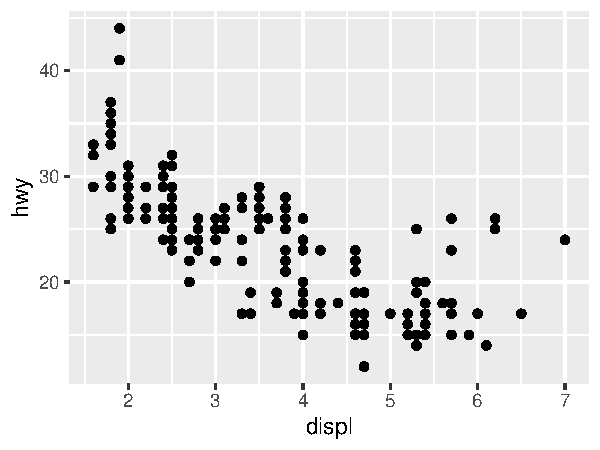
\includegraphics{_main_files/figure-latex/first-plot-1.pdf}
\caption{\label{fig:first-plot}ggplot2의 산점도}
\end{figure}

패키지 \texttt{ggplot2}에서 그래프 작성은 함수 \texttt{ggplot()}으로 시작한다.
이 함수는 우선 그래프 작성에 사용되는 데이터를 입력 요소 \texttt{data}에서 지정하는데,
데이터는 반드시 데이터 프레임이어야 한다. 또한 이 함수는 그래프가 작성될 좌표계(coordinate system)를 작성하고,
이어서 작성될 그래프를 기다리는 역할을 한다. 따라서 함수 \texttt{ggplot()}만으로는 실질적인
그래프가 작성되지 않는다.

실질적인 그래프는 이어진 함수 \texttt{geom\_point()}로 작성된다. 패키지 \texttt{ggplot2}에서는 하나
또는 여러 개의 레이어(layer)들이 겹쳐져서 그래프가 완성되는데, Figure \ref{fig:first-plot}에는 점으로
이루어진 하나의 레이어만이 사용되었다. 레이어를 추가하는 \texttt{geom} 함수에는 \texttt{geom\_point()}
외에도 다양한 함수들이 있으며, 앞으로 계속 소개될 것이다.

또한 \texttt{geom} 함수에는 입력 요소 \texttt{mapping}이 있는데, 이것은 항상 함수 \texttt{aes()}와 함께 사용된다.
매핑(mapping)은 데이터와 그래프의 시각적 요소(aesthetic)를 서로 연결시키는 것으로,
함수 \texttt{aes()}의 입력 요소 x와 y는 X축과 Y축에 각각의 변수를 연결시키는 역할을 하고 있다.

\begin{itemize}
\tightlist
\item
  \texttt{ggplot2}에서 그래프 작성의 최소 요소
\end{itemize}

패키지 \texttt{ggplot2}에서 그래프를 작성하기 위해서는 반드시 따라야 할 법칙이 있다.
이 법칙은 '그래프의 문법'이라고 불리는 것으로서 모든 그래프 작성에서 일정하게 적용되기 때문에
익숙해지기만 한다면 복잡한 형태의 그래프도 쉽게 작성할 수 있게 된다.
패키지 \texttt{ggplot2}에서 그래프를 작성하기 위한 3가지 최소 요소는 \texttt{\textless{}Data\textgreater{}}, \texttt{\textless{}Geom\_Function\textgreater{}},
그리고 \texttt{\textless{}Mappings\textgreater{}}로써 다음과 같은 형식을 취해야 한다.

\begin{verbatim}
> ggplot(data = <Data>) +
+   <Geom_FUnction>(mapping = aes(<Mappings>))
\end{verbatim}

\texttt{\textless{}Data\textgreater{}}는 그래프 작성에 사용될 데이터 프레임을 지정하는 것이고,
\texttt{\textless{}Geom\_Function\textgreater{}}은 geom 함수 중 하나를 지정하는 것으로써 레이어를 작성한다.
여러 개의 레이어를 겹치기 위해서는 필요한 여러 개의 geom 함수를 덧셈 기호로 연결하면 된다.
\texttt{\textless{}Mappings\textgreater{}}는 다양한 시각적 요소(크기, 모양, 색깔 등)와 데이터를 연결하는 것이다.

3가지의 필수 요소 외에도 다양한 그래프를 작성하기 위해서는 몇 가지 기본 요소가 더
필요하다. 앞으로 하나하나 살펴보도록 하겠다.

  \bibliography{book.bib,packages.bib}

\end{document}
